\subsection{Diagramas de clases de package com.example.prueba3.Views}

La arquitectura de nuestra aplicación móvil se organiza en paquetes bien definidos para una clara separación de responsabilidades. Dentro de este esquema, el paquete `com.example.prueba3.Views`, que contiene nuestros ViewModels, se erige como un componente central y fundamental.

Los ViewModels son elementos clave en la construcción de interfaces de usuario robustas y reactivas. Su función primordial es actuar como intermediarios estratégicos entre las `Pantallas` (implementadas como Composables en el paquete `Pantallas`), y la lógica de negocio o las fuentes de datos. Un ViewModel se encarga de exponer los datos necesarios para su `Pantalla` asociada de una manera que sea óptima para la interfaz de usuario, garantizando que el estado de la UI persista a través de cambios de configuración del dispositivo, como rotaciones o reconstrucciones de la actividad.

A continuación se presentara las clases que conforman a package.example.prueba3.Views:


\subsection{Diagrama de clases de package.example.prueba3.Views parte 1}

La Figura \ref{fig:Views1} muestra la primera parte del diagrama de clases de package.example.prueba3.Views.

\begin{figure}[htbp!]
	\begin{center}
		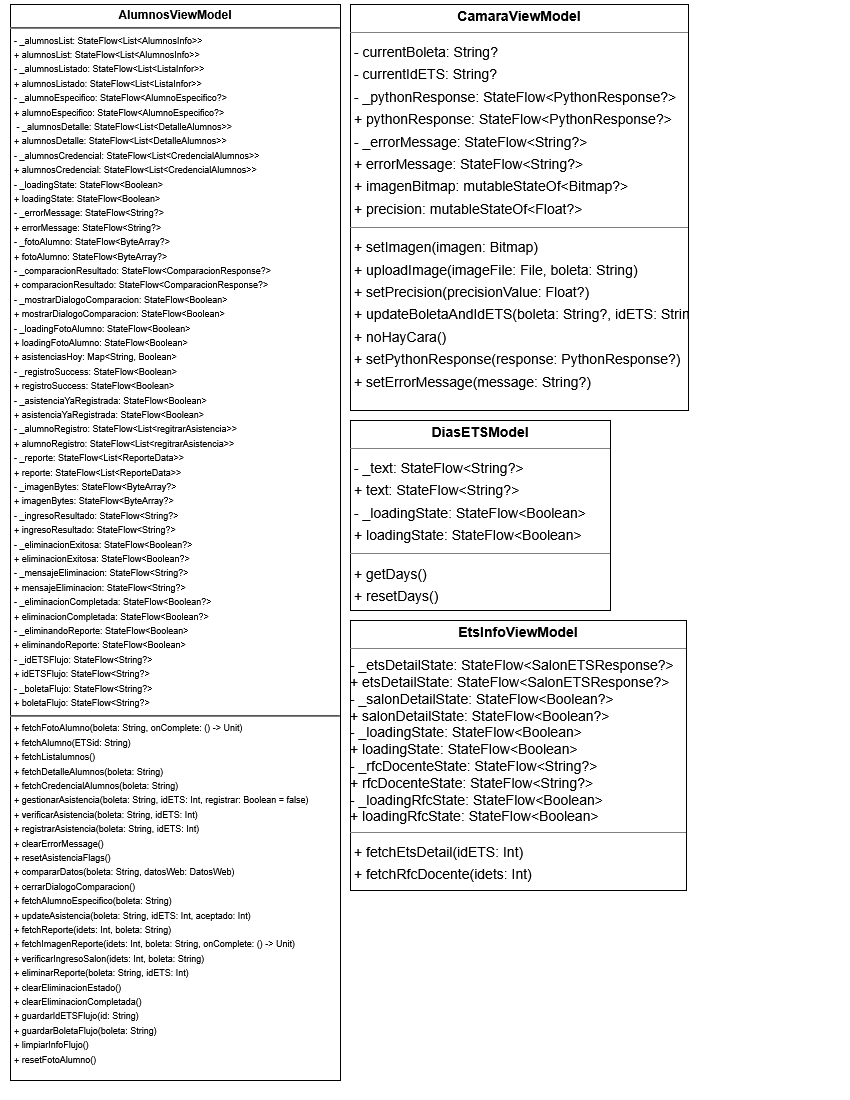
\includegraphics[width=0.75\textwidth]{DiagramasMoviles/DCM (7)}
		\caption{Diagrama de clases para package.example.prueba3.Views parte 1.}
		\label{fig:Views1}
	\end{center}
\end{figure}

\newpage

\subsection{Diagrama de clases de package.example.prueba3.Views parte 2}

La Figura \ref{fig:Views2} muestra la segunda parte del diagrama de clases de package.example.prueba3.Views.

\begin{figure}[htbp!]
	\begin{center}
		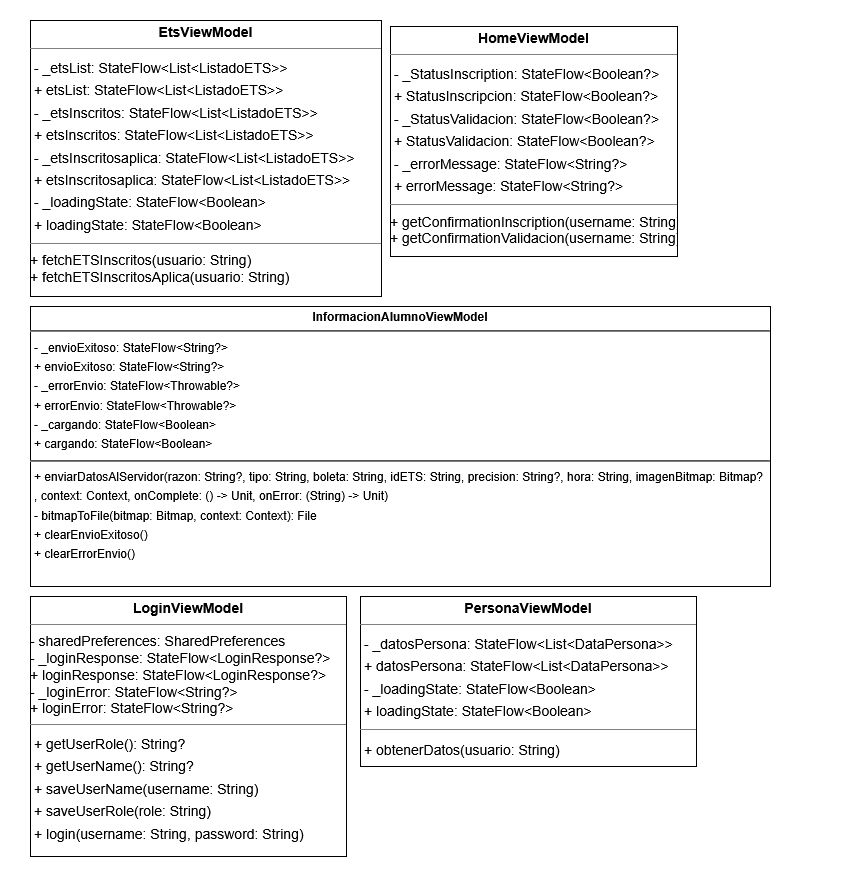
\includegraphics[width=0.75\textwidth]{DiagramasMoviles/DCM (8)}
		\caption{Diagrama de clases para package.example.prueba3.Views parte 2.}
		\label{fig:Views2}
	\end{center}
\end{figure}

\newpage

\subsection{Diagrama de clases de package.example.prueba3.Views parte 3}

La Figura \ref{fig:Views3} muestra la tercer parte del diagrama de clases de package.example.prueba3.Views.

\begin{figure}[htbp!]
	\begin{center}
		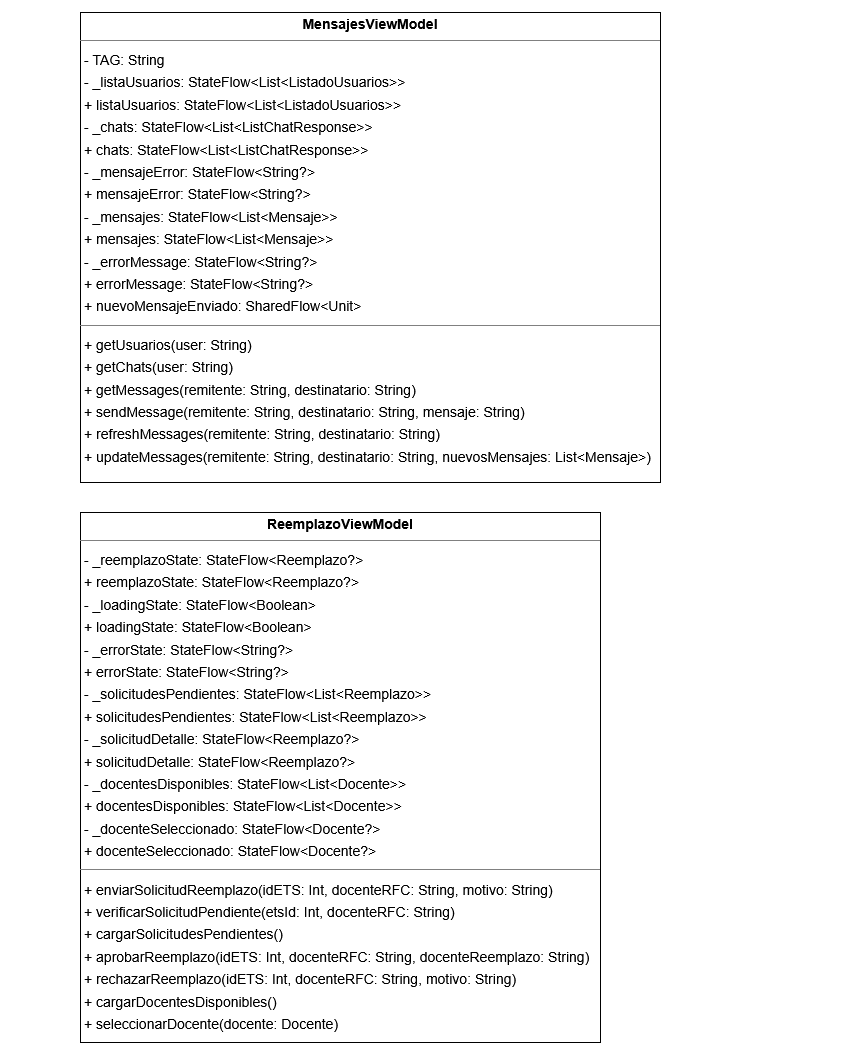
\includegraphics[width=0.75\textwidth]{DiagramasMoviles/DCM (9)}
		\caption{Diagrama de clases para package.example.prueba3.Views parte 3.}
		\label{fig:Views3}
	\end{center}
\end{figure}

\newpage